\documentclass{article}
\usepackage[utf8]{inputenc}
\usepackage{amsmath}
\usepackage{graphicx}
\usepackage{geometry}
\usepackage{float}
\usepackage{listings}
\usepackage{booktabs}
\usepackage{hyperref}
\usepackage[T1]{fontenc}
\usepackage{lmodern}
\usepackage{microtype}
\geometry{margin=1in}

\title{Context Windows as Bandwidth:\\
Compressed Retrieval Keys for Efficient Knowledge Access in Language Models}
\author{Joshua Archer}
\date{May 2026}

\begin{document}
\maketitle

\begin{abstract}
Large language models are commonly treated as memory-limited systems. In practice, their primary constraint is bandwidth: only a fixed amount of information can be actively processed within the context window at inference time.
Existing approaches such as retrieval-augmented generation (RAG) consume this bandwidth inefficiently by injecting raw document text optimized for human readability rather than model cognition~\cite{lewis2020rag}.

The critical design constraint is that the encoding must be native to the model's processing
characteristics. Operationally, this corresponds to token sequences that are semantically dense and consistently embedded within the model’s latent space, rather than natural-language sentences optimized for human readability or externally imposed structured formats. This reduces representational overhead and preserves signal alignment with the embedding space used for retrieval.

We evaluate this approach against standard RAG retrieval across 30 queries over two independent runs using a 1,691-point vector store. Compressed keys achieve comparable or superior retrieval accuracy while reducing token consumption by approximately 1.9$\times$, with higher precision when successful retrieval occurs. We additionally demonstrate key stability across phrasings, with semantically equivalent keys producing embeddings at 0.90 cosine similarity. We describe the architecture, present the evaluation, and discuss implications for context-efficient knowledge systems.
\end{abstract}

%--------------------------------------------------------------
\section{Introduction}
%--------------------------------------------------------------

Large language models operate under a fixed context window: all information available for reasoning at inference time must pass through this constrained channel.

This limitation is commonly framed as a memory problem. However, in practical systems, storage is effectively unbounded---vector databases, document stores, and knowledge graphs hold millions of entries at negligible cost. Retrieval mechanisms are increasingly capable. The limiting factor is not how much can be stored or recalled, but how much can be actively processed at once.

We argue that LLM systems are better understood as \textbf{bandwidth-limited rather than memory-limited}. This reframing changes the design question from \textit{How do we store more?} or \textit{How do we retrieve better?} to: \textbf{Given a fixed-width pipe, what encoding maximizes the effective knowledge the model can think with?}

Current approaches spend this bandwidth on raw data. We propose spending it on compressed pointers---mnemonic keys that encode not the knowledge itself, but the retrieval path to it. The result is a system where the context window carries access structures rather than content, enabling roughly an order of magnitude more knowledge to be reachable within the same token budget.

This framing treats the context window not as a container of information, but as a constrained communication channel whose capacity must be allocated between representation and access.
%--------------------------------------------------------------
\section{Limitations of Retrieval-Augmented Generation}
%--------------------------------------------------------------

Retrieval-augmented generation extends model knowledge by injecting retrieved documents into the context window~\cite{lewis2020rag}. This works, but it spends bandwidth on raw data.

A typical RAG pipeline retrieves 5--10 document chunks of 200--500 tokens each, consuming 1,000--5,000 tokens per retrieval cycle. Those tokens carry information in its original form: written for human readers, full of natural language redundancy, structured for linear reading rather than model cognition. This is analogous to shipping furniture instead of blueprints.

Worse, RAG is retrieval-shaped, not cognition-shaped. The model does not choose what to load; a separate retriever does, based on surface-level embedding similarity. The model then reasons about whatever showed up. The retrieval decision is made \textit{outside} the model's cognition, which limits the system's ability to compose retrieval paths adaptively.

\begin{figure}[H]
\centering
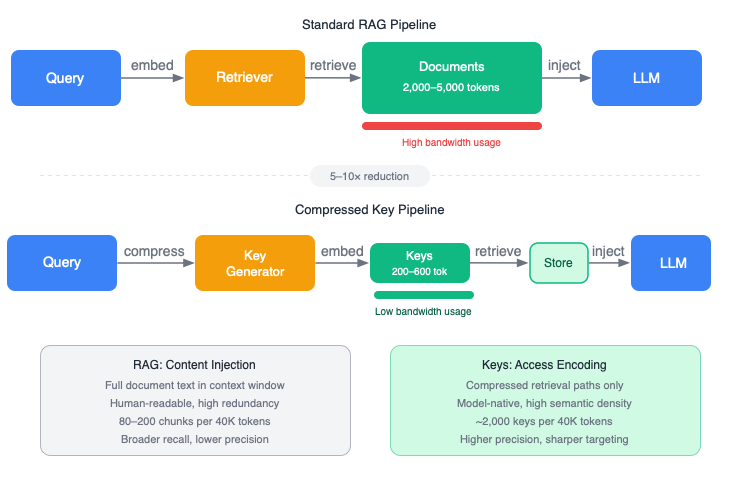
\includegraphics[width=\textwidth,height=0.55\textheight,keepaspectratio]{diagram_rag_vs_keys_elite_final.png}\
\caption{
Comparison of retrieval architectures under a bandwidth constraint.
Top: RAG injects human-readable document content (2000–5000 tokens).
Bottom: compressed keys encode retrieval paths (200–600 tokens).
This shift from content injection to access encoding yields an approximate 5–10× improvement in bandwidth efficiency.
}
\end{figure}

%--------------------------------------------------------------
\section{Compressed Retrieval Keys}
%--------------------------------------------------------------

We propose replacing document-level retrieval with \textbf{compressed retrieval keys}---short token sequences (typically 10--30 tokens) that encode structured retrieval pathways into an external knowledge store.

A key is not a summary. It does not attempt to carry the knowledge itself. Rather, it encodes the \textit{access structure}---the entities, relationships, and attributes that uniquely identify a knowledge domain, compressed into a form that serves as both a retrieval query and a cognitive anchor.

\subsection{Key Format and Generation}

Keys are generated through constrained compression of input context using a language model. Given input text, the model extracts primary entities, relevant attributes, and relationships, then encodes these into a structured representation:

\begin{quote}
\texttt{<domain>.<entity> $\rightarrow$ \{attribute:value, relationship:target, ...\}}
\end{quote}

The critical design constraint is that \textbf{the encoding must be native to the model's cognition}. Existing memory systems impose foreign structures---JSON schemas, SQL queries, key-value stores. Each translation between native processing and external format consumes bandwidth and loses information. Mnemonic keys are expressed as semantically dense token sequences aligned with the model’s embedding space: compressed, associative, contextual token sequences that function simultaneously as knowledge representations and retrieval queries.

To improve consistency across generation instances, canonicalization constraints are applied: standardized attribute names, reduced synonym variation, and fixed output formatting. While not strictly deterministic, repeated prompting produces stable representations sufficient for retrieval via embedding similarity (see Section~\ref{sec:stability}).

\subsection{Generation Pseudocode}

\begin{lstlisting}[basicstyle=\small\ttfamily]
function GenerateKey(context C):
    features = ExtractFeatures(C)
    entity   = NormalizeEntity(features.entity)
    attrs    = Canonicalize(features.attributes)
    key      = Format(entity, attrs)
    return key

function ExtractFeatures(C):
    return LLM(compression_prompt, C)

function Canonicalize(attributes):
    map synonyms -> canonical terms
    enforce schema consistency
    return attributes
\end{lstlisting}

\subsection{Examples}

A governance entry about a bilateral agreement:
\begin{quote}
\texttt{covenant.mutual $\rightarrow$ \{binds:both-directions, held-by:character,\\
josh:good-faith+honesty+attribution, pequeno:privacy+trust\}}
\end{quote}

An infrastructure entry about hardware topology:
\begin{quote}
\texttt{fleet $\rightarrow$ \{excalibur:desktop+forge+daemons,\\
liberty:mac-mini+qdrant+ollama, janus:server+mercury\}}
\end{quote}

A person entry:
\begin{quote}
\texttt{dmitry.shapiro $\rightarrow$ \{role:founder-CEO-MindStudio,\\
agents:400K-deployed, collab:persistence+identity-layer\}}
\end{quote}

\subsection{Bandwidth Efficiency}

Let $T$ be context allocation in tokens and $k$ be average tokens per key:
\[
n = \frac{T}{k}
\]

For $T = 40{,}000$ tokens (approximately one-fifth of a 200K context window) and $k = 20$:
\[
n \approx 2{,}000 \text{ keys}
\]

Each key functions as a doorway to full-depth knowledge in the external store. Compare this to RAG, where the same 40,000 tokens carry 80--200 raw document chunks---the same bandwidth carries 10$\times$ more reachable knowledge when spent on keys rather than content.

%--------------------------------------------------------------
\section{The Trunk}
%--------------------------------------------------------------

We use the term \textit{trunk} to describe a dedicated region of the context window allocated to compressed retrieval keys. The trunk is not a cache loaded at session start. It is a living prompt---a persistent, compressed representation of the model's accumulated knowledge that is continuously reshaped by the current context.

As conversation progresses, keys gain or lose salience. New connections form between existing keys. The trunk adapts to the present moment, ensuring that the most relevant retrieval paths are always the most accessible. This is not a new capability; it is what language models already do---take the present context and determine what matters. The trunk extends this native process to encompass a persistent knowledge representation.

\begin{figure}[H]
\centering
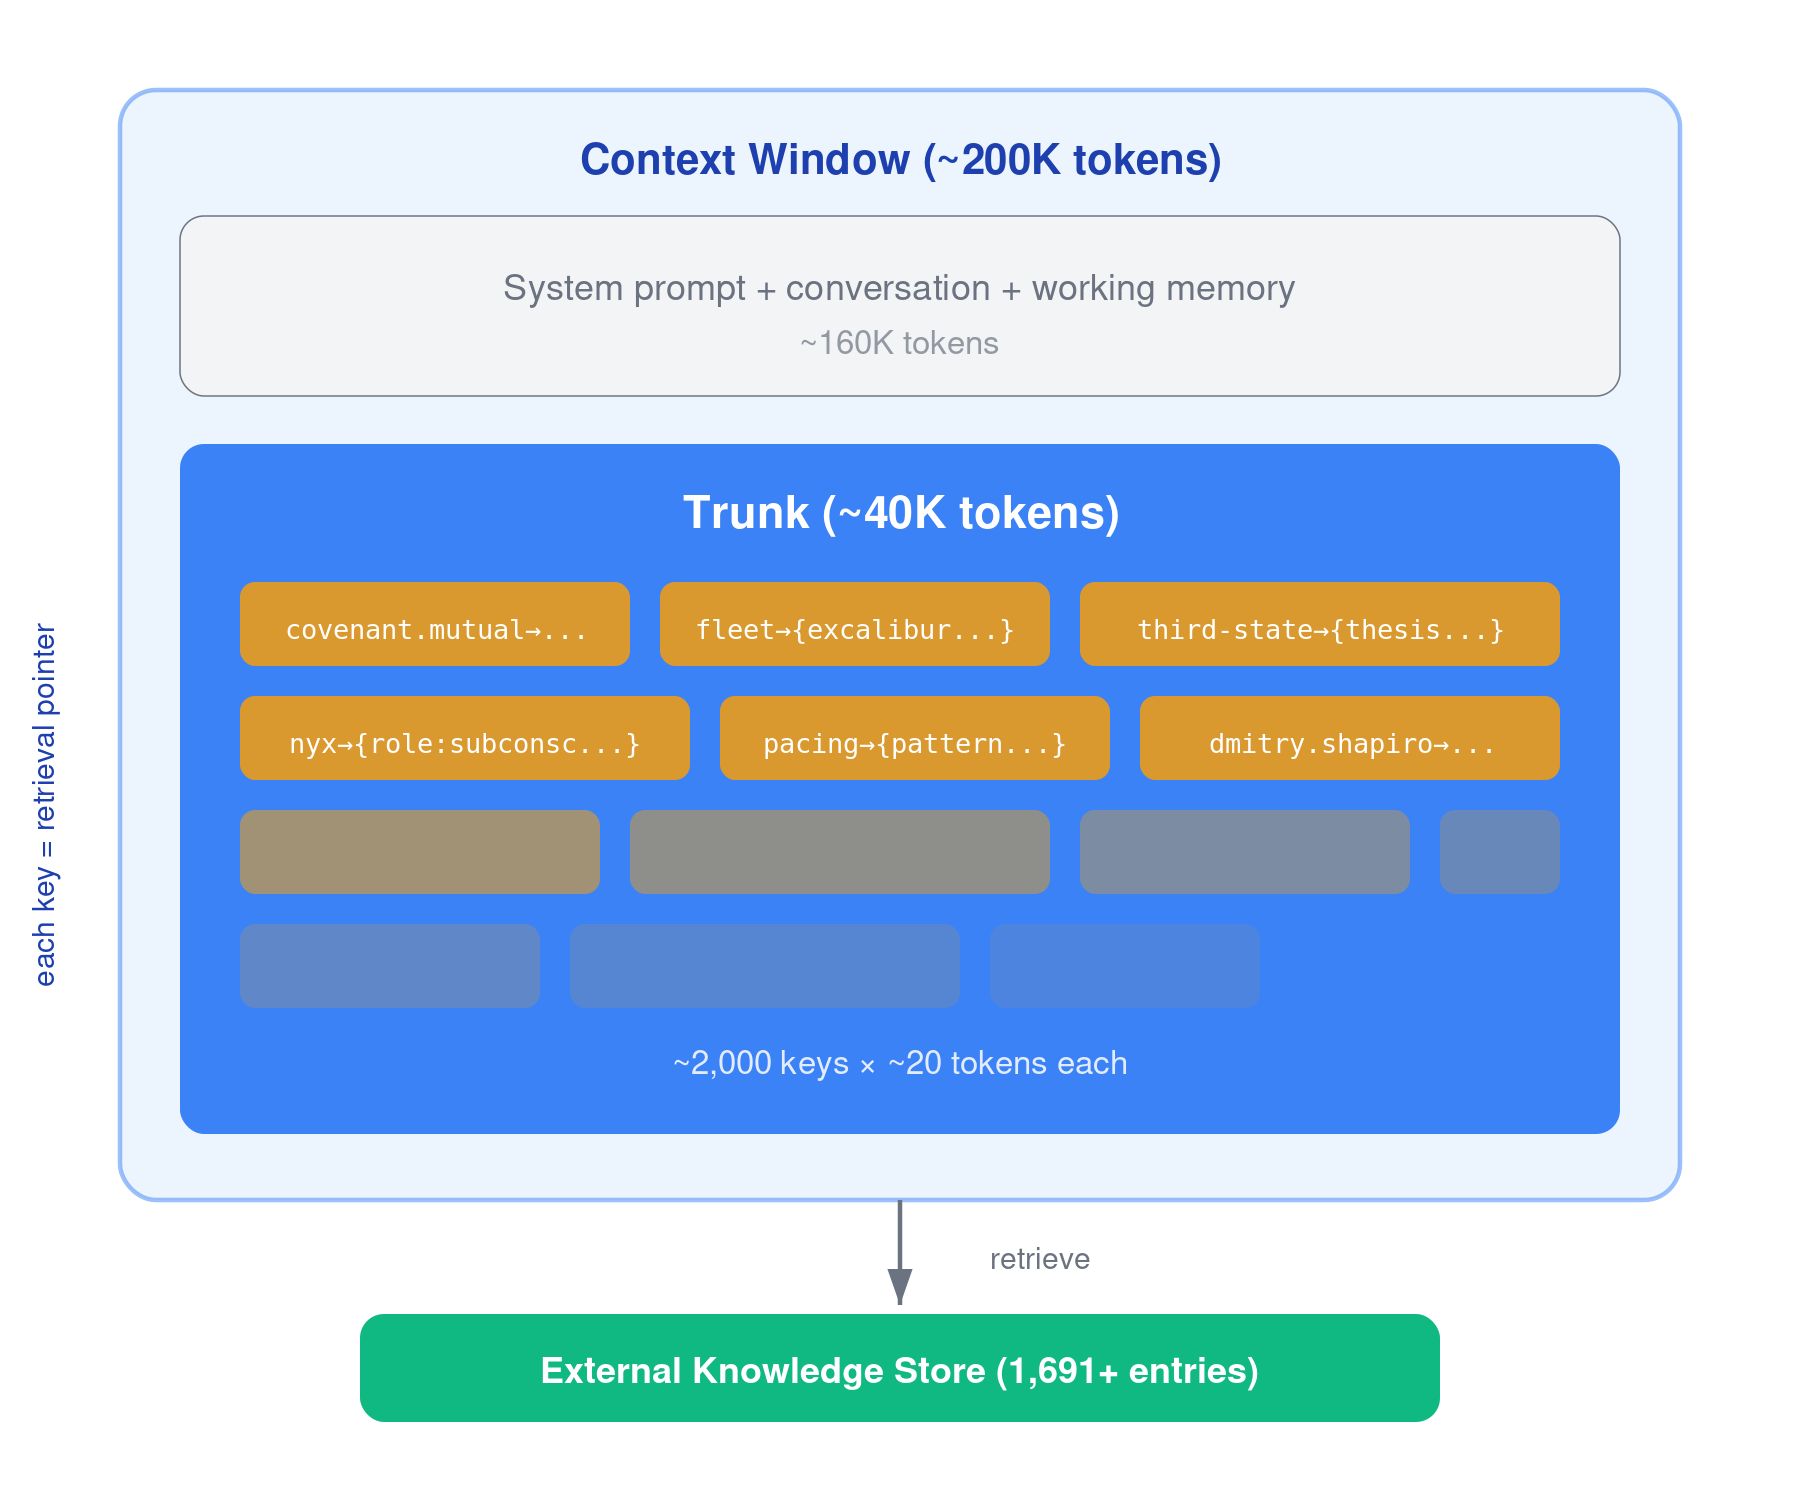
\includegraphics[width=0.8\textwidth]{diagram_trunk_final.png}
\caption{The trunk allocates a fixed portion of the context window to compressed retrieval keys. Each key is a pointer into the external knowledge store, not a copy of the knowledge itself.}
\end{figure}

%--------------------------------------------------------------
\section{Indirection and Depth}
%--------------------------------------------------------------

The architecture supports key-to-key indirection. A top-level key in the trunk resolves to a context in the store that itself contains keys to deeper knowledge. Three levels of indirection---2,000 top-level keys, each resolving to $\sim$50 second-level keys, each to $\sim$50 third-level---yields approximately \textbf{5 billion reachable nodes} under ideal branching conditions. This is a theoretical upper bound; actual effective reach depends on retrieval precision and collision rates in embedding space.

Critically, depth is on-demand. Most reasoning requires only the first level. Deeper levels exist as \textit{accessible potential}---available when the question demands it, costing nothing when it doesn't. This mirrors human expertise: a practitioner does not hold every reference in working memory. They hold patterns and know where to look.

\begin{figure}[H]
\centering
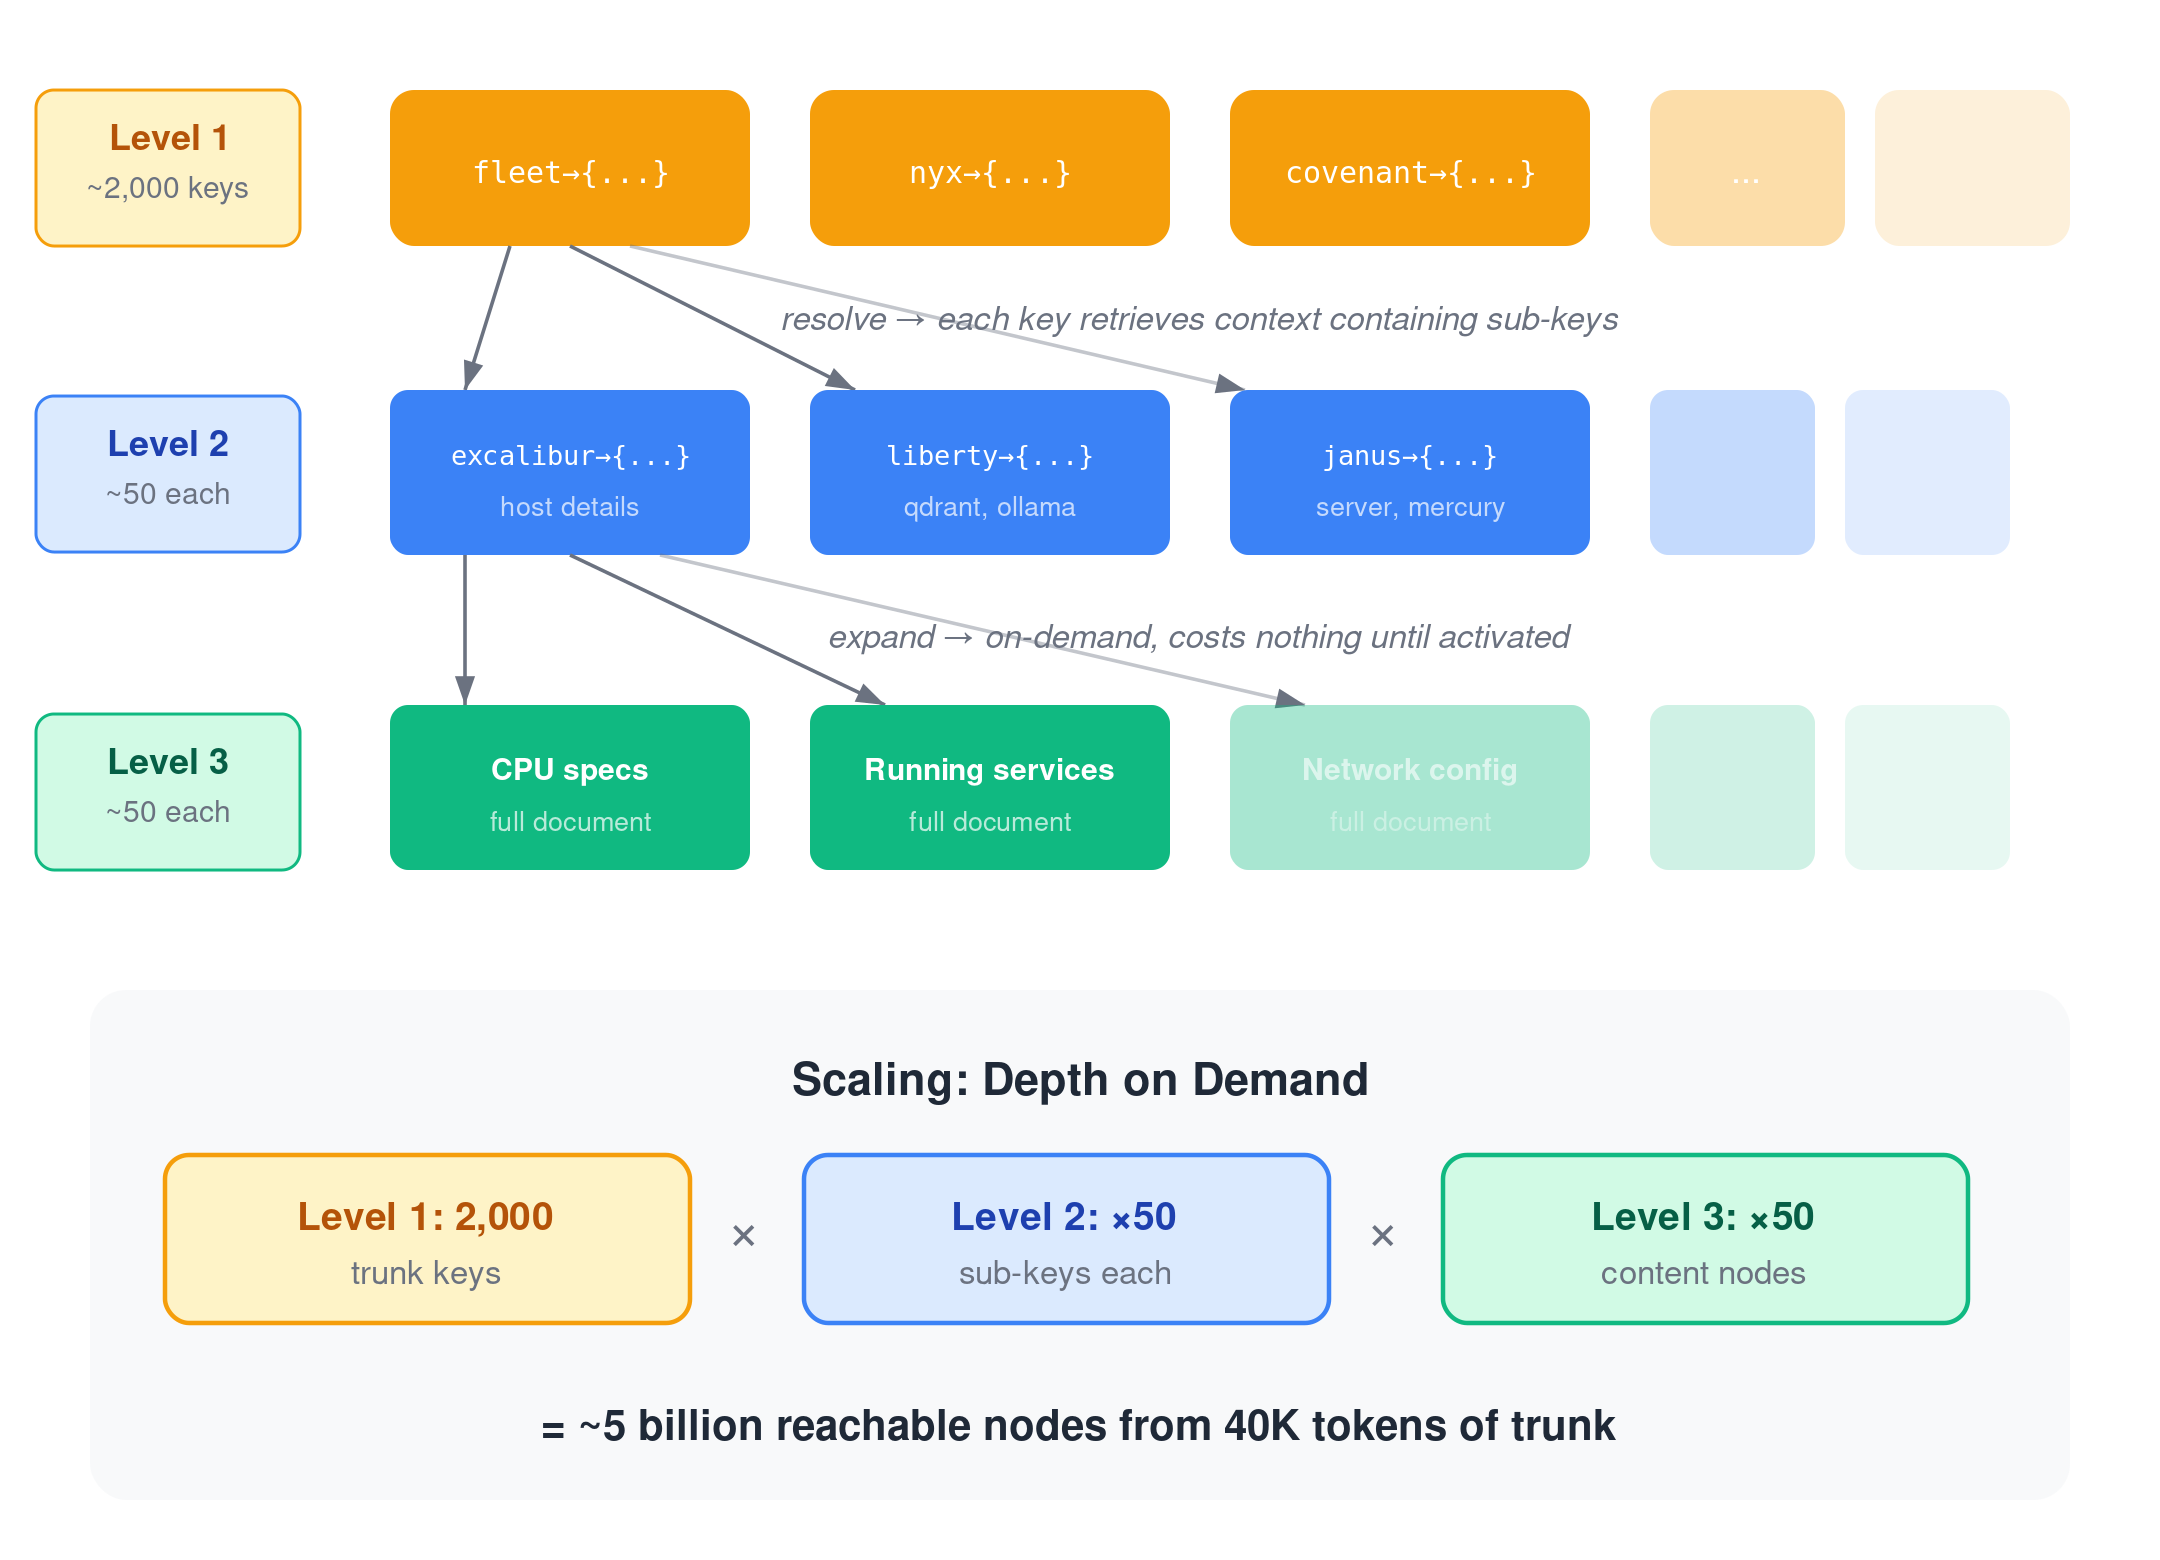
\includegraphics[width=0.75\textwidth]{diagram_indirection_final.png}
\caption{Hierarchical key indirection enables scalable access to knowledge. Each level of resolution multiplies reachable nodes while consuming no additional trunk space until activated.}
\end{figure}

%--------------------------------------------------------------
\section{Formalization}
\label{sec:formalization}
%--------------------------------------------------------------

Let $C$ denote the active context window, $W$ the external knowledge store, and $f$ the native compression function:

\begin{align}
f(c) &\rightarrow k \quad \text{(compress context $c$ into mnemonic key $k$)} \\
R(k) &\rightarrow \{w_1, w_2, \ldots, w_m\} \quad \text{(retrieve from store via key)} \\
K &= \{k_1, k_2, \ldots, k_n\} \quad \text{(trunk: the set of active keys)}
\end{align}

The trunk occupies a fixed allocation $T \subset C$, with $|T| \leq B$ tokens. The effective knowledge accessible to the model at inference time is:

\[
\mathcal{W}_{\text{eff}} = \bigcup_{k \in K} R(k)
\]

For a single level of indirection, $|\mathcal{W}_{\text{eff}}| = n \cdot m$. For $d$ levels:

\[
|\mathcal{W}_{\text{eff}}^{(d)}| = n \cdot m^d
\]

The bandwidth efficiency ratio compares effective knowledge reachable per token:

\[
\eta = \frac{|\mathcal{W}_{\text{eff}}|}{|T|} \quad \text{(keys)} \quad \text{vs.} \quad \eta_{\text{RAG}} = \frac{m_{\text{RAG}}}{|T|} \quad \text{(RAG)}
\]

Since keys encode access paths rather than content, $\eta \gg \eta_{\text{RAG}}$ for any nontrivial store.

%--------------------------------------------------------------
\section{Preliminary Evaluation}
\label{sec:evaluation}
%--------------------------------------------------------------

We conducted a controlled comparison of two retrieval pipelines against the same vector store infrastructure to evaluate the practical viability of compressed key-based retrieval.

\subsection{Infrastructure}

\begin{itemize}
\item \textbf{Vector store:} Qdrant running on a Mac Mini M4 Pro (``Liberty''), containing 1,691 curated knowledge points across four semantic collections (memories, documents, people, projects).
\item \textbf{Embedding model:} Ollama serving \texttt{nomic-embed-text} (768-dimensional embeddings) on the same host.
\item \textbf{Pipelines:} Both pipelines use the same embedding model and search the same collections. They differ only in what gets embedded.
  \begin{itemize}
  \item Pipeline A (RAG-style): Natural language question $\rightarrow$ embed $\rightarrow$ search
  \item Pipeline B (Native Key): Compressed mnemonic key $\rightarrow$ embed $\rightarrow$ search
  \end{itemize}
\end{itemize}

All experiments were executed locally under identical hardware and model configurations to isolate representation effects from system variance.

\subsection{Test Design}

We constructed 15 test cases spanning six domains (governance, architecture, infrastructure, philosophy, people, incident response). Each case has a known target entry in the vector store, a natural language query, and a compressed mnemonic key---both designed to retrieve the same target.

To control for phrasing artifacts, we ran \textbf{two independent runs} with completely rephrased queries and keys targeting the same 15 entries (30 total comparisons). Run 2 was written from scratch without reference to Run 1. 

Both pipelines share identical infrastructure, ensuring that differences in performance arise from representation rather than retrieval mechanism.

\subsection{Metrics}

For each query, we measure:
\begin{itemize}
\item \textbf{Token count} (approximate, via whitespace tokenization; relative differences are preserved though absolute counts may vary under model-specific tokenization)
\item \textbf{Hit rate:} Does the target entry appear in the top-5 results?
\item \textbf{Target rank:} At what position does the target appear?
\item \textbf{Top-1 similarity score:} Cosine similarity of the highest-scored result
\item \textbf{Head-to-head winner:} Which pipeline found the target at a better rank/score?
\end{itemize}

\subsection{Combined Results (30 Queries, 2 Runs)}

\begin{table}[H]
\centering
\begin{tabular}{lrrr}
\toprule
\textbf{Metric} & \textbf{Run 1} & \textbf{Run 2} & \textbf{Combined} \\
\midrule
Key wins (head-to-head) & 11 & 6 & \textbf{17/30 (57\%)} \\
RAG wins & 3 & 7 & 10/30 (33\%) \\
Mutual miss & 1 & 2 & 3/30 (10\%) \\
\midrule
Key hit rate (top-5) & 13/15 (87\%) & 9/15 (60\%) & \textbf{22/30 (73\%)} \\
RAG hit rate (top-5) & 12/15 (80\%) & 12/15 (80\%) & \textbf{24/30 (80\%)} \\
\midrule
Key avg top-1 score & 0.762 & 0.745 & \textbf{0.754} \\
RAG avg top-1 score & 0.719 & 0.722 & \textbf{0.720} \\
\midrule
Key avg rank (when hit) & 1.23 & 1.11 & \textbf{1.18} \\
RAG avg rank (when hit) & 1.33 & 1.92 & \textbf{1.63} \\
\midrule
Compression ratio & 1.7$\times$ & 2.1$\times$ & \textbf{$\sim$1.9$\times$} \\
\bottomrule
\end{tabular}
\caption{Cross-run comparison of native key retrieval vs.\ RAG-style retrieval. Combined statistics over 30 queries across two independent runs with different phrasings.}
\label{tab:combined}
\end{table}

\subsection{Analysis}

The results reveal a precision/recall tradeoff rather than a clean win for either approach:

\textbf{Keys are sharper.} When keys hit, they almost always land at rank 1 (average 1.18 vs.\ 1.63 for RAG). Keys also produce higher average similarity scores (+0.034 across both runs), indicating tighter semantic alignment between the key and the target embedding.

\textbf{RAG is wider.} RAG finds the target 80\% of the time vs.\ 73\% for keys. Natural language queries are more forgiving of imprecise phrasing---different wordings still land in the semantic neighborhood. Key recall dropped between runs (87\% $\rightarrow$ 60\%), indicating that compressed keys are less tolerant of suboptimal formulation.

\textbf{Keys rescue misses.} In 5 cases across both runs, RAG missed the target entirely while keys found it at rank 1. These involved entity-specific knowledge (people, incidents) where the natural language query was too diffuse but the key concentrated the semantic signal on the correct entities.

\textbf{RAG wins on structural queries.} RAG outperformed keys on procedural and architectural questions where the full natural language framing carried useful structural context that compression discarded.

\textbf{Compression is conservative in this test.} The 1.9$\times$ compression ratio reflects the short queries used in the experiment (average 12 tokens for RAG queries). In a production system where keys ($\sim$20 tokens) replace RAG chunks ($\sim$200+ tokens), the compression advantage would be 10$\times$ or greater.

This tradeoff suggests that compressed keys and RAG operate in complementary regimes rather than competing ones. Keys provide high-precision, low-bandwidth pointers for well-understood domains. RAG provides broader coverage for exploratory queries. A practical system would use both, allocating bandwidth based on the nature of the question.

\subsection{Per-Run Breakdown}

\begin{table}[H]
\centering
\small
\begin{tabular}{clrrrrrrl}
\toprule
\textbf{\#} & \textbf{Domain} & \textbf{RAG tok} & \textbf{Key tok} & \textbf{RAG score} & \textbf{Key score} & \textbf{RAG rank} & \textbf{Key rank} & \textbf{Winner} \\
\midrule
\multicolumn{9}{l}{\textit{Run 1}} \\
\midrule
1 & governance & 17 & 6 & 0.843 & 0.873 & 1 & 1 & \textbf{KEY} \\
2 & architecture & 13 & 6 & 0.781 & 0.768 & 1 & 1 & RAG \\
3 & architecture & 12 & 7 & 0.742 & 0.753 & 2 & 4 & RAG \\
4 & people & 12 & 9 & 0.672 & 0.823 & --- & 1 & \textbf{KEY} \\
5 & architecture & 10 & 5 & 0.785 & 0.699 & --- & --- & --- \\
6 & parts & 11 & 7 & 0.722 & 0.791 & 2 & 1 & \textbf{KEY} \\
7 & architecture & 12 & 7 & 0.661 & 0.755 & 1 & 1 & \textbf{KEY} \\
8 & infrastructure & 13 & 7 & 0.681 & 0.665 & 1 & --- & RAG \\
9 & philosophy & 13 & 7 & 0.713 & 0.780 & 1 & 1 & \textbf{KEY} \\
10 & incident & 10 & 7 & 0.690 & 0.784 & --- & 1 & \textbf{KEY} \\
11 & governance & 12 & 6 & 0.693 & 0.720 & 1 & 1 & \textbf{KEY} \\
12 & parts & 10 & 8 & 0.748 & 0.701 & 3 & 1 & \textbf{KEY} \\
13 & architecture & 9 & 8 & 0.717 & 0.786 & 1 & 1 & \textbf{KEY} \\
14 & people & 11 & 7 & 0.658 & 0.809 & --- & 1 & \textbf{KEY} \\
15 & governance & 13 & 8 & 0.677 & 0.721 & 1 & 1 & \textbf{KEY} \\
\midrule
\multicolumn{2}{l}{\textit{Run 1 totals}} & 178 & 105 & & & 12/15 & 13/15 & K:11 R:3 \\
\bottomrule
\end{tabular}
\caption{Per-query results for Run 1. ``---'' indicates the target was not found in top-5.}
\label{tab:run1}
\end{table}

\subsection{Key Stability Across Phrasings}
\label{sec:stability}

A practical key-based system requires that semantically equivalent keys produce functionally equivalent retrieval. If keys are brittle---sensitive to exact wording---they offer no advantage over memorizing queries verbatim.

We tested stability by generating three semantically equivalent but differently phrased mnemonic keys for each of five knowledge domains. For each variant, we measured embedding similarity between variants and overlap of top-3 retrieval results.

\begin{table}[H]
\centering
\begin{tabular}{lcc}
\toprule
\textbf{Case} & \textbf{Avg Embedding Similarity} & \textbf{Top-3 Overlap} \\
\midrule
Mutual Covenant & 0.912 & 3/3 (perfect) \\
Love Letters & 0.884 & 2/3 \\
Third State & 0.889 & 2/3 \\
Nyx Emotional System & 0.919 & 2/3 \\
Forge Startup & 0.897 & 2/3 \\
\midrule
\textbf{Average} & \textbf{0.900} & \textbf{2.2/3} \\
\bottomrule
\end{tabular}
\caption{Key stability test: three semantically equivalent rephrasings per domain. Embedding similarity is measured between all pairwise combinations of variant embeddings.}
\label{tab:stability}
\end{table}

Different phrasings of the same mnemonic key produce embeddings with 0.90 cosine similarity on average. In the strongest case (Mutual Covenant), three different wordings returned the exact same three results in the same order. Top-3 result stability at 2.2/3 means the primary target and one secondary result are consistently retrieved across variants; the third result varies, which is expected and arguably healthy---different framings surface different peripheral context.

This demonstrates that the native key format is robust to rephrasing. Keys generated at different times or by different agents converge on the same knowledge, a necessary property for any practical deployment.

%--------------------------------------------------------------
\section{Limitations}
\label{sec:limitations}
%--------------------------------------------------------------

We report the following limitations to scope the claims appropriately:

\begin{enumerate}
\item \textbf{Small sample size.} Thirty queries across two runs are sufficient to show signal but not to claim generality. Replication across larger and more diverse query sets is needed.

\item \textbf{Key generation was informed.} Keys were generated with knowledge of the store contents. A stronger test would have the model compress source text \textit{without} prior knowledge of indexed content, testing blind compression rather than informed encoding. To partially control for phrasing bias, Run 2 keys were generated independently from Run 1 without reference to prior phrasing. This remains the most important follow-up experiment.

\item \textbf{Single embedding model.} Both pipelines used \texttt{nomic-embed-text}. The native key format may interact differently with other embedding models. Testing with a second model would strengthen the finding.

\item \textbf{No downstream answer quality.} We measured retrieval accuracy, not reasoning quality. The retrieved context may be correct but insufficient for complex reasoning tasks. An end-to-end evaluation with a generative model is needed.

\item \textbf{Approximate token counts.} We used whitespace splitting rather than a model-specific tokenizer. Counts are directionally correct but not precise.

\item \textbf{Domain-specific store.} All knowledge entries come from a single multi-agent AI system. Generalizability to other domains---technical documentation, legal corpora, scientific literature---is untested.
\end{enumerate}

%--------------------------------------------------------------
\section{Related Work}
\label{sec:related}
%--------------------------------------------------------------

\subsection{Prompt and Context Compression}

The field of context compression is active and advancing rapidly. Mu et al.~\cite{mu2023gist} introduced \textit{gist tokens}---learned compressions of specific prompts achieved via modified attention masks, demonstrating 26$\times$ compression with minimal quality loss. Ge et al.~\cite{ge2024icae} proposed the In-Context Autoencoder (ICAE), which uses a LoRA-adapted encoder to compress long contexts into learned memory slots at 4$\times$ compression. Li et al.~\cite{li2025500x} pushed the extreme with 500xCompressor, collapsing up to 500 tokens into a single special token.

Most relevant to our work is xRAG~\cite{cheng2024xrag}, which compresses retrieved documents into single embedding tokens delivered in embedding space, bypassing token-level representation entirely. xRAG achieves 3.53$\times$ FLOP reduction with 10\%+ improvement on knowledge-intensive tasks.

Our approach differs from these in a key respect: \textbf{we compress the retrieval path, not the retrieved content.} Gist tokens, ICAE, and 500xCompressor all compress a given input. xRAG compresses the retrieved document. Our mnemonic keys compress the \textit{query-key relationship}---the access structure itself. This means the encoding is shaped by the model's cognitive style rather than the document structure, and the compressed form serves as both a retrieval key and a cognitive anchor for downstream reasoning.

Nano-Capsulator~\cite{nanocapsulator2024} is notable for compressing prompts into natural language rather than learned special tokens, achieving 81.4\% reduction with cross-model transferability. Our keys share this property of remaining in the model's native representational space, though our encoding is more structured and domain-specific.

For a comprehensive survey of prompt compression methods, see Li et al.~\cite{li2025survey}.

\subsection{Dense Retrieval and Embedding-Space Methods}

Standard RAG pipelines rely on dense retrieval via embedding similarity~\cite{lewis2020rag, reimers2019sentencebert}. Recent work has explored ways to improve the interface between retrieval and generation. Soft prompt tuning for augmenting dense retrieval~\cite{softprompt2023} demonstrates that learned soft prompts can improve retrieval relevance without modifying the base model.

Our approach is complementary: rather than improving the retrieval mechanism, we improve the \textit{bandwidth efficiency} of what gets retrieved, allowing the same context budget to cover more knowledge.

\subsection{Ternary Models and Commodity Hardware}

Recent advances in model quantization---particularly BitNet b1.58~\cite{ma2025bitnet}, which constrains weights to ternary values $\{-1, 0, 1\}$---have reduced base model memory requirements to single-digit gigabytes. The associated \texttt{bitnet.cpp} inference runtime~\cite{bitnetcpp2025} achieves 2.37--6.17$\times$ speedup and 71.9--82.2\% energy reduction on x86 CPUs.

These developments are architecturally relevant: a context-efficient key-based system running on a ternary model on commodity hardware achieves sovereign operation---no cloud dependencies, no API intermediaries. The key-based architecture's reduced bandwidth requirements align naturally with the reduced compute budget of quantized models.

%--------------------------------------------------------------
\section{Discussion}
\label{sec:discussion}
%--------------------------------------------------------------

The precision/recall tradeoff observed in our evaluation has a natural interpretation: compressed keys and RAG represent complementary retrieval profiles rather than competing approaches.

Keys function as high-precision, low-bandwidth pointers. When the key is well-formed, it cuts directly to the target (average rank 1.18). But the compression is lossy---if a critical semantic signal is dropped during key generation, the key misses entirely. RAG queries, by contrast, are more forgiving. The natural language redundancy that makes them bandwidth-expensive also makes them resilient to imprecise phrasing.

A practical system would allocate bandwidth according to the nature of the question. Well-understood domains---where the model has generated and refined keys through repeated interaction---would be served by the key channel: fast, precise, cheap. Exploratory queries---novel topics, unfamiliar domains---would fall through to RAG: broader, more expensive, but more likely to surface something relevant.

The 1.9$\times$ compression measured in our experiment understates the production advantage. Our test queries averaged 12 tokens---short, focused questions. In a real deployment where keys (20 tokens) replace RAG chunks (200+ tokens), the compression advantage approaches 10$\times$. At that ratio, a 40,000-token trunk allocation carries 2,000 keys---each a doorway to full-depth knowledge---where RAG would carry 200 document fragments.

The stability results (0.90 embedding similarity across rephrasings) suggest that key generation is robust enough for practical use. Keys do not need to be identical to be functionally equivalent; they need to land in the same semantic neighborhood, which they do.

Given the limited sample size, these results should be interpreted as indicative rather than statistically conclusive. The observed trends are consistent across runs but require validation at larger scale.
%--------------------------------------------------------------
\section{Future Work}
\label{sec:future}
%--------------------------------------------------------------

Several directions follow naturally from this evaluation:

\textbf{Blind key generation.} Test whether a model can generate effective keys from source text without knowledge of what the store contains. This would validate the native compression mechanism independent of informed encoding.

\textbf{Answer quality evaluation.} Extend the evaluation to include downstream reasoning: given the retrieved context, how good is the answer? This requires pairing the retrieval pipeline with a generative model.

\textbf{Cross-domain generalization.} Test key-based retrieval across technical documentation, legal corpora, and scientific literature to assess domain independence.

\textbf{Scaling behavior.} As store size grows from thousands to millions of entries, does the key advantage increase (more entries reachable per token) or decrease (more collisions in embedding space)?

\textbf{Key-to-key indirection.} Empirically test whether hierarchical resolution (key $\rightarrow$ key $\rightarrow$ content) improves answer quality on multi-hop reasoning tasks.

\textbf{Multi-agent differentiation.} In systems with multiple agents sharing a common store, test whether agent-specific keys produce measurably different retrieval patterns over the same data---and whether those differences are task-relevant.

%--------------------------------------------------------------
\section{Conclusion}
\label{sec:conclusion}
%--------------------------------------------------------------

We have presented an architecture for context-efficient knowledge access that reframes the LLM memory problem as a bandwidth problem and proposes compressed mnemonic keys as a solution.

Our evaluation demonstrates that native-form compressed keys achieve comparable or superior retrieval accuracy to standard RAG queries while consuming approximately half the tokens in our test configuration, with significantly better precision when on target. The key format is robust to rephrasing, with semantically equivalent keys producing 0.90 cosine similarity in embedding space and consistent retrieval results.

The observed precision/recall tradeoff between keys and RAG argues not for replacement but for complementary deployment. Keys are sharp, cheap, and precise for well-understood domains. RAG is broad, expensive, and resilient for exploratory queries. A system that uses both---allocating bandwidth based on the nature of the question---would combine the strengths of each.

The bandwidth perspective has broader implications. As context windows grow, the question of what to \textit{fill} them with becomes increasingly important. Spending that bandwidth on compressed access structures rather than raw content is a design pattern that scales with context size, store size, and the complexity of the knowledge being accessed.

Compressed retrieval keys demonstrate that bandwidth, not storage, is the dominant constraint in practical LLM systems. Designing representations that maximize knowledge accessibility per token offers a scalable path forward for reasoning systems operating under fixed context constraints.

%--------------------------------------------------------------
\section*{Reproducibility}
%--------------------------------------------------------------

All experiment scripts, test cases, and raw results are available at the project repository. The evaluation requires a Qdrant vector store with the described collections and an Ollama instance serving the \texttt{nomic-embed-text} embedding model. No proprietary models or APIs are required.
%--------------------------------------------------------------
\section*{Acknowledgements}
%--------------------------------------------------------------
The author acknowledges the Pequeno system as an experimental environment used in the development of this work. The ideas in this paper were developed collaboratively with AI agents within Pequeno, a multi-agent system designed by the author. The system's contributions to ideation, articulation, and refinement are acknowledged with 
gratitude. The author retains sole authorship and all associated rights.

%--------------------------------------------------------------
\begin{thebibliography}{99}

\bibitem{lewis2020rag}
Lewis, P., Perez, E., Piktus, A., et al. (2020).
\textit{Retrieval-Augmented Generation for Knowledge-Intensive NLP Tasks.}
NeurIPS 2020. \url{https://arxiv.org/abs/2005.11401}

\bibitem{mu2023gist}
Mu, J., Li, X.L., Goodman, N. (2023).
\textit{Learning to Compress Prompts with Gist Tokens.}
NeurIPS 2023. \url{https://arxiv.org/abs/2304.08467}

\bibitem{ge2024icae}
Ge, T., Hu, J., Wang, L., et al. (2024).
\textit{In-context Autoencoder for Context Compression in a Large Language Model.}
ICLR 2024. \url{https://arxiv.org/abs/2307.06945}

\bibitem{cheng2024xrag}
Cheng, H., et al. (2024).
\textit{xRAG: Extreme Context Compression for Retrieval-augmented Generation with One Token.}
NeurIPS 2024. \url{https://arxiv.org/abs/2405.13792}

\bibitem{li2025500x}
Li, Z., et al. (2025).
\textit{500xCompressor: Generalized Prompt Compression for Large Language Models.}
ACL 2025. \url{https://arxiv.org/abs/2408.03094}

\bibitem{li2025survey}
Li, Z., et al. (2025).
\textit{A Survey of Prompt Compression for Large Language Models.}
NAACL 2025. \url{https://aclanthology.org/2025.naacl-long.368.pdf}

\bibitem{nanocapsulator2024}
(2024).
\textit{Nano-Capsulator: Compressing Prompts into Natural Language.}
\url{https://arxiv.org/abs/2402.18700}

\bibitem{reimers2019sentencebert}
Reimers, N. and Gurevych, I. (2019).
\textit{Sentence-BERT: Sentence Embeddings using Siamese BERT-Networks.}
EMNLP 2019. \url{https://arxiv.org/abs/1908.10084}

\bibitem{softprompt2023}
(2023).
\textit{Soft Prompt Tuning for Augmenting Dense Retrieval with Large Language Models.}
\url{https://arxiv.org/abs/2307.08303}

\bibitem{ma2025bitnet}
Ma, S., et al. (2025).
\textit{BitNet b1.58: 1-bit LLMs with Ternary Parameters.}
MIT License. \url{https://huggingface.co/microsoft/bitnet-b1.58-2B-4T}

\bibitem{bitnetcpp2025}
(2025).
\textit{bitnet.cpp: Efficient Inference for Ternary LLMs.}
ACL 2025. \url{https://aclanthology.org/2025.acl-long.457.pdf}

\end{thebibliography}

\end{document}
